%%=============================================================================
%% LaTeX sjabloon voor bachelorproef, HoGent Bedrijf en Organisatie
%% Opleiding Toegepaste Informatica
%%=============================================================================

\documentclass[pdftex,a4paper,12pt,twoside]{report}

% TODO: Let op: dit sjabloon is ontworpen om dubbelzijdig af te drukken, met
% asymmetrische marges. Voor enkelzijdig, verwijder ``twoside'' hierboven.

%%=============================================================================
%% LaTeX sjabloon voor de bachelorproef, HoGent Bedrijf en Organisatie
%% Opleiding toegepaste informatica
%%
%% Structuur en algemene vormgeving. Meestal hoef je hier niets te wijzigen.
%%
%% Auteur: Bert Van Vreckem <bert.vanvreckem@hogent.be>
%% Licentie: CC-BY https://creativecommons.org/licenses/by/4.0/
%%=============================================================================

%%---------- Packages ---------------------------------------------------------

\usepackage[utf8]{inputenc}  % Accenten gebruiken in tekst (vb. é ipv \'e)
\usepackage{amsfonts}        % AMS math packages: extra wiskundige
\usepackage{amsmath}         %   symbolen (o.a. getallen-
\usepackage{amssymb}         %   verzamelingen N, R, Z, Q, etc.)
\usepackage[english,dutch]{babel}    % Taalinstellingen: woordsplitsingen,
                             %  commando's voor speciale karakters
                             %  ("dutch" voor NL)
\usepackage{iflang}
\usepackage{eurosym}         % Euro-symbool €
\usepackage{geometry}
\usepackage{graphicx}        % Invoegen van tekeningen
\usepackage[pdftex,bookmarks=true]{hyperref}
                             % PDF krijgt klikbare links & verwijzingen,
                             %  inhoudstafel

\usepackage{listings}        % Broncode mooi opmaken
\usepackage[T1]{fontenc}
\usepackage[scaled]{beramono}

\usepackage{color}
\definecolor{bluekeywords}{rgb}{0.13,0.13,1}
\definecolor{greencomments}{rgb}{0,0.5,0}
\definecolor{redstrings}{rgb}{0.9,0,0}

\usepackage{listings}
\lstset{language=[Sharp]C,
showspaces=false,
showtabs=false,
breaklines=true,
showstringspaces=false,
breakatwhitespace=true,
escapeinside={(*@}{@*)},
commentstyle=\color{greencomments},
keywordstyle=\color{bluekeywords}\bfseries,
stringstyle=\color{redstrings},
basicstyle=\ttfamily
}
\usepackage{multirow}        % Tekst over verschillende cellen in tabellen
\usepackage{rotating}        % Tabellen en figuren roteren
\usepackage{natbib}          % Betere bibliografiestijlen
\usepackage{fancyhdr}        % Pagina-opmaak met hoofd- en voettekst

\usepackage[T1]{fontenc}     % Ivm lettertypes
\usepackage{lmodern}
\usepackage{textcomp}

\usepackage{etoolbox}
\usepackage{lipsum}          % Voor vultekst (lorem ipsum)

%%---------- Layout -----------------------------------------------------------

\pagestyle{fancy}                % Hoofdingen invoegen
\renewcommand{\sectionmark}[1]{} % Enkel hoofdstuktitel in hoofding, geen
                                 % sectietitel (vermijd overlap)

% Leeg blad
\newcommand{\emptypage}{
\newpage
\thispagestyle{empty}
\mbox{}
\newpage
}

% Gebruik een schreefloos lettertype ipv het "oubollig" uitziende
% Computer Modern
\renewcommand{\familydefault}{\sfdefault}

%%---------- Broncode (Java) --------------------------------------------------
% Commando voor invoegen Java-broncodebestanden (dank aan Niels Corneille)
% Gebruik:
%   \codefragment{source/MijnKlasse.java}{Uitleg bij de code}
%
% Je kan dit aanpassen aan de taal die je zelf het meeste gebruikt in je
% bachelorproef.
\newcommand{\codefragment}[2]{ \lstset{%
  language=java,
  breaklines=true,
  float=th,
  caption={#2},
  basicstyle=\scriptsize,
  frame=single,
  extendedchars=\true
}
\lstinputlisting{#1}}


%%---------- Voorblad ---------------------------------------------------------

\newcommand{\inserttitlepage}{%
\begin{titlepage}
  \newgeometry{top=2cm,bottom=1.5cm,left=1.5cm,right=1.5cm}
  \begin{center}

    \begingroup
    \rmfamily
    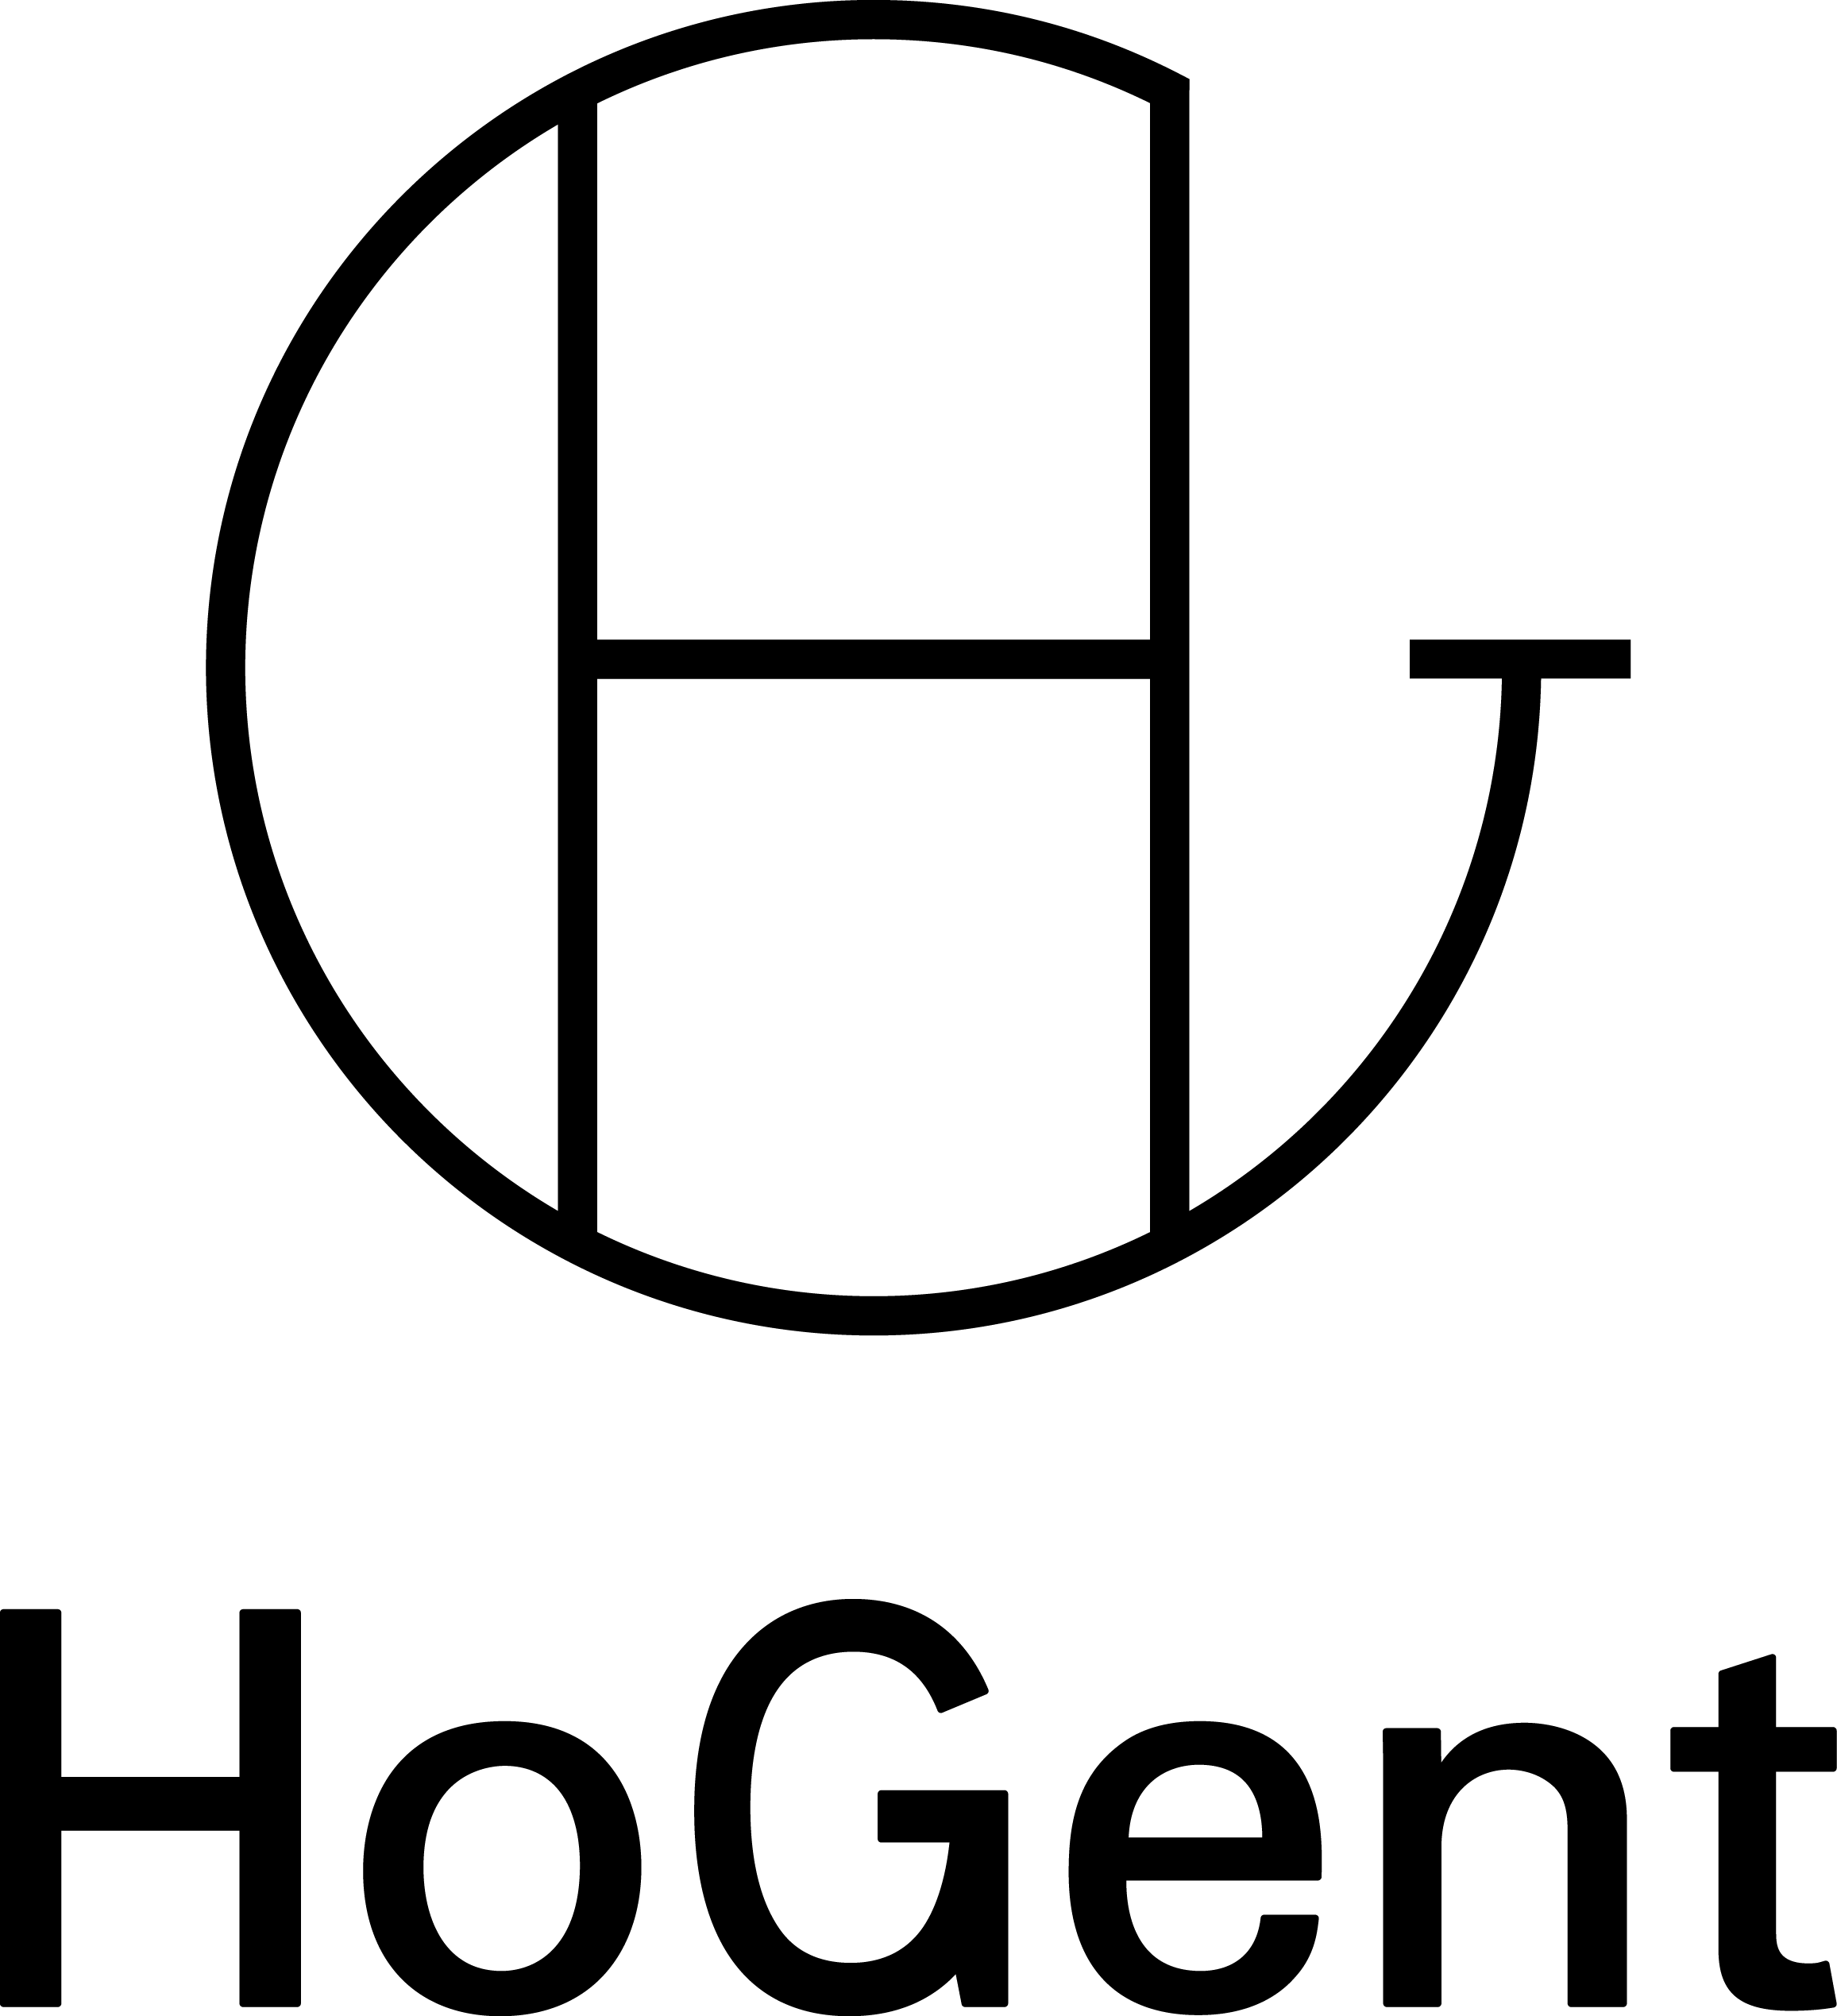
\includegraphics[width=2.5cm]{img/HG-beeldmerk-woordmerk}\\[.5cm]
    Faculteit Bedrijf en Organisatie\\[3cm]
    \titel
    \vfill
    \student\\[3.5cm]
    Scriptie voorgedragen tot het bekomen van de graad van\\professionele bachelor in de toegepaste informatica\\[2cm]
    Promotor:\\
    \promotor\\
    \ifdefempty{\copromotor}{\vspace{2.5cm}}{Co-promotor:\\\copromotor\\[2.5cm]}
    Instelling: \instelling\\[.5cm]
    Academiejaar: \academiejaar\\[.5cm]
    \ifcase \examenperiode \or Eerste \or Tweede \else Derde \fi examenperiode
    \endgroup

  \end{center}
  \restoregeometry
\end{titlepage}
  \emptypage
\begin{titlepage}
  \newgeometry{top=5.35cm,bottom=1.5cm,left=1.5cm,right=1.5cm}
  \begin{center}

    \begingroup
    \rmfamily
    \IfLanguageName{dutch}{Faculteit Bedrijf en Organisatie}{Faculty of Business and Information Management}\\[3cm]
    \titel
    \vfill
    \student\\[3.5cm]
    \IfLanguageName{dutch}{Scriptie voorgedragen tot het bekomen van de graad van\\professionele bachelor in de toegepaste informatica}{Thesis submitted in partial fulfillment of the requirements for the degree of\\professional bachelor of applied computer science}\\[2cm]
    Promotor:\\
    \promotor\\
    \ifdefempty{\copromotor}{\vspace{2.5cm}}{Co-promotor:\\\copromotor\\[2.5cm]}
    \IfLanguageName{dutch}{Instelling}{Institution}: \instelling\\[.5cm]
    \IfLanguageName{dutch}{Academiejaar}{Academic year}: \academiejaar\\[.5cm]
    \IfLanguageName{dutch}{%
    \ifcase \examenperiode \or Eerste \or Tweede \else Derde \fi examenperiode}{%
    \ifcase \examenperiode \or First \or Second \else Third \fi examination period}
    \endgroup

  \end{center}
  \restoregeometry
\end{titlepage}
}


%%---------- Documenteigenschappen --------------------------------------------
%% TODO: Vul dit aan met je eigen info:

% Je eigen naam
\newcommand{\student}{Piet Pieters}

% De naam van je promotor (lector van de opleiding)
\newcommand{\promotor}{Bert Van Vreckem}

% De naam van je co-promotor. Als je promotor ook je opdrachtgever is en je
% dus ook inhoudelijk begeleidt, mag je dit leeg laten.
\newcommand{\copromotor}{}

% Indien je bachelorproef in opdracht van/in samenwerking met een bedrijf of
% externe organisatie geschreven is, geef je hier de naam. Zoniet laat je dit
% zoals het is.
\newcommand{\instelling}{---}

% De titel van het rapport/bachelorproef
\newcommand{\titel}{Titel}

% Datum van indienen (gebruik telkens de deadline, ook al geef je eerder af)
\newcommand{\datum}{27 mei 2016}

% Academiejaar
\newcommand{\academiejaar}{2015-2016}

% Examenperiode
%  - 1e semester = 1e examenperiode => 1
%  - 2e semester = 2e examenperiode => 2
%  - tweede zit  = 3e examenperiode => 3
\newcommand{\examenperiode}{2}

%%=============================================================================
%% Inhoud document
%%=============================================================================

\begin{document}

%% Als je je bachelorproef in het Engels schrijft, haal dan onderstaande regel
%% uit commentaar. Let op: de tekst op de voorkaft blijft in het Nederlands, en
%% dat is ook de bedoeling!
%\selectlanguage{english}

\inserttitlepage

%%=============================================================================
%% Samenvatting
%%=============================================================================

%% TODO: De "abstract" of samenvatting is een kernachtige (~ 1 blz. voor een
%% thesis) synthese van het document.
%%
%% Deze aspecten moeten zeker aan bod komen:
%% - Context: waarom is dit werk belangrijk?
%% - Nood: waarom moest dit onderzocht worden?
%% - Taak: wat heb je precies gedaan?
%% - Object: wat staat in dit document geschreven?
%% - Resultaat: wat was het resultaat?
%% - Conclusie: wat is/zijn de belangrijkste conclusie(s)?
%% - Perspectief: blijven er nog vragen open die in de toekomst nog kunnen
%%    onderzocht worden? Wat is een mogelijk vervolg voor jouw onderzoek?
%%
%% LET OP! Een samenvatting is GEEN voorwoord!

%%---------- Nederlandse samenvatting -----------------------------------------
%%
%% TODO: Als je je bachelorproef in het Engels schrijft, moet je eerst een
%% Nederlandse samenvatting invoegen. Haal daarvoor onderstaande code uit
%% commentaar.
%% Wie zijn bachelorproef in het Nederlands schrijft, kan dit negeren en heel
%% deze sectie verwijderen.


%%---------- Samenvatting -----------------------------------------------------
%%
%% De samenvatting in de hoofdtaal van het document

\begin{abstract}
  %%\lipsum[1-4]

  Deze bachelorproef heeft als doel de ontwikkelaar op basis van onderzoek naar ontwikkeltijd, kosten, snelheid en gegevensverbruik
  te helpen in de keuze tussen een cross platforme mobiele applicatie en responsive website. Dit omdat er vandaag de dag weinig artikels
  ter beschikking zijn waarin een gefundeerde keuze wordt gemaakt voor 1 van beide vormen van toepassingen.

  Dit werk is tot stand gekomen in verschillende fases. Zo werd er eerst een literatuuronderzoek verricht naar eerdere vergelijkende
  studie tussen cross platforme mobiele apps en responsive websites.

  Na het vastleggen van de casus werd er gekozen voor Visual Studio als ontwikkelingomgeving, waarna de ontwikkeling van beide toepassingen volgde. Eens de ontwikkeling afgerond was, werden de tijden voor
  opstarten, inloggen en gegevens ophalen gemeten samen met de hoeveelheid gegevens die dit met zich meebrengt. Dit om nadien een
  gefundeerde conclusie te vormen op basis van snelheid, gegevensverbruik, kosten. Dit alles zonder caching van data in de mobiele applicatie.

  Uit de resultaten van het onderzoek kwam naar voor dat indien men het gegevensverbruik van de toepassing een belangrijk kenmerk vindt, men
  beter kiest voor de mobiele applicatie. Voor de snelheid van de toepassing, heeft bij Android
  de responsive website een duidelijk voordeel ten opzicht van de mobiele applicatie. Bij windowsphone was mobiele applicatie sneller.
  In het iOS-project is wegens tijdgebrek enkel het inloggen gedeeltelijk geïmplementeerd. Hierop werden geen testen uitgevoerd.

  Verder worden ook de kosten om beide toepassingen te hosten in rekening genomen. voor de mobiele applicatie komt dit voor de web api € 92,56 per maand.
  Hierbij moeten nog de kosten voor publicatie in de applicatiewinkel meegerekend worden. Voor android is dit eenmalig 25 dollar. Voor windowsphone is
  dit € 16,98 (19 dollar) voor een individueel account en € 88,50 (99 dollar) voor een bedrijfsaccount. De kost voor de iOS-applicatie te publiceren komt op 99 dollar per jaar.
  Indien deze kosten van belang zijn, kiest men beter voor de responsive webapplicatie. Dit omdat hier enkel de € 92,56 per maand erbij komt.
  Dit naast de kosten voor een macOS-toestel om de iOS-applicatie op te testen.

  De snelheid van ontwikkeling is een criterium dat ook in rekening werd gebracht in deze vergelijkende studie.
  Hierbij was het resultaat dat bij de responsive website sneller tot een gebruiksklaar eindproduct kon komen.
  Dit terwijl men bij de mobiele applicatie drie afzonderlijke deelprojecten moest maken. De uitgebereide resultaten en conclusies
  worden meer in detail toegelicht in de scriptie.



\end{abstract}

%%=============================================================================
%% Voorwoord
%%=============================================================================

\chapter*{Voorwoord}
\label{ch:voorwoord}

%% TODO:
%% Het voorwoord is het enige deel van de bachelorproef waar je vanuit je
%% eigen standpunt (``ik-vorm'') mag schrijven. Je kan hier bv. motiveren
%% waarom jij het onderwerp wil bespreken.
%% Vergeet ook niet te bedanken wie je geholpen/gesteund/... heeft

In deze bachelorproef worden de verschillen in performantie tussen een cross-platforme mobiele applicatie en responsive website onderzocht.
De keuze voor dit onderwerp is gekomen na een opdrachtswijziging in de stage van het vorige academiejaar (2015-2016).

Toen werd er na een kostenanalyse van een cross-platforme mobiele applicatie beslist om over te schakelen op een responsive website.
Het was dan dat mijn interesse om dit uitgebereider te onderzoeken, getriggerd werd.

Deze vergelijkende studie en proof-of-concept in functie van een doelbewuste keuze tussen een cross platforme mobiele applicatie en
een mobiele website werd gevoerd tussen februari 2017 en mei 2017 bij de ICT-afdeling van de Gentse Politie.

Daarom wens ik ook mijn dank te betuigen aan mijn co-promotor Jeroen Gevenois om mij steeds bij te staan tijden mijn onderzoeken en voor
het beantwoorden van mijn vragen tijdens het ontwikkelen van beide toepassingen.
op mijn vragen tijdens het ontwikkelen van beide toepassingen.

Ook wil ik ook Matthias Vercaemst bedanken om mij te helpen met de verschillende netwerken-vragen die ik had tijdens het onderzoek.

Ook diensthoofd Ruben Vansevenant zou ik graag willen vermelden in mijn bedankingen omdat hij mij de kans te geven om deze bachelorproef uit te werken.

Verder wil ik ook mijn promotor Koen Hoof bedanken voor de steeds opbouwende feedback en de stipte opvolging van deze bachelorproef tijdens de afgelopen maanden.
Deze feedback hielp mij om telkens weer dit werk te verbeteren.

Tot slot bedank ik nog mijn Gon-Begeleider Elke Van Paemel voor de steun tijdens het schrijven van de bachelorproef.


\tableofcontents

%% Als je een lijst van afkortingen of termen wil toevoegen, dan hoort die
%% hier thuis. Gebruik bijvoorbeeld de ``glossaries'' package.

%%---------- Kern -------------------------------------------------------------


%%=============================================================================
%% Inleiding
%%=============================================================================

\chapter{Inleiding}
\label{ch:inleiding}

%% De inleiding moet de lezer alle nodige informatie verschaffen om het onderwerp te begrijpen zonder nog externe werken te moeten raadplegen \citep{Pollefliet2011}. Dit is een doorlopende tekst die gebaseerd is op al wat je over het onderwerp gelezen hebt (literatuuronderzoek).

%% Je verwijst bij elke bewering die je doet, vakterm die je introduceert, enz. naar je bronnen.
%% In \LaTeX{} kan dat met het commando \texttt{$\backslash${cite\{\}}} of \texttt{$\backslash${citep\{\}}}.
%%Als argument van het commando geef je de ``sleutel'' van een ``record'' in een bibliografische databank in het Bib\TeX{}-formaat
%% (een tekstbestand). Als je expliciet naar de auteur verwijst in de zin, gebruik je \texttt{$\backslash${}cite\{\}}.
%% Soms wil je de auteur niet expliciet vernoemen, dan gebruik je \texttt{$\backslash${}citep\{\}}.
%%Hieronder een voorbeeld van elk.

\section{Stand van zaken}
\label{sec:stand-van-zaken}

%% TODO: deze sectie (die je kan opsplitsen in verschillende secties) bevat je
%% literatuurstudie. Vergeet niet telkens je bronnen te vermelden!
In de vakliteratuur zijn er vandaag diverse artikelen te vinden over een vergelijkende studie tussen mobiele applicatie
en responsive webapplicaties. Meeste onderzoeken die tot nu toe gevoerd zijn, zijn echter een beperkte lijst van kenmerken die aangeven wanneer men het best voor welke optie kiest.
Dit zonder dat hier wetenschappelijk onderzoek aan vooraf ging.

Toch zijn deze wetenschappelijke artikelen beschikbaar. Zo onderzocht \cite{albuquerque2015}
in het artikel 'CROSS PLATFORM APP A COMPARATIVE STUDY' de voornaamste reden om te kiezen voor enerzijds de mobiele
applicatie en anderzijds de responsive website.

De belangrijkste redenen uit het onderzoek om te kiezen voor een cross-platform mobiele applicatie zijn de volgende:
\begin{itemize}
  \item{Performantie}
  \item{User Interfaces in de lijn van het besturingssysteem}
  \item{Distributie via de app stores}
  \item{Push notificaties}
\end{itemize}

In de vakliteratuur haalt men voor de hoofdzakelijkste redenen om te kiezen voor een responsive webapplicatie, de volgende aan:
\begin{itemize}
  \item{Eenvoudige ondersteuning voor meerdere systemen}
  \item{Het publiceren van de toepassing}
\end{itemize}



\section{Probleemstelling en Onderzoeksvragen}
\label{sec:onderzoeksvragen}

%% TODO:
%% Uit je probleemstelling moet duidelijk zijn dat je onderzoek een meerwaarde
%% heeft voor een concrete doelgroep (bv. een bedrijf).
%%
%% Wees zo concreet mogelijk bij het formuleren van je
%% onderzoeksvra(a)g(en). Een onderzoeksvraag is trouwens iets waar nog
%% niemand op dit moment een antwoord heeft (voor zover je kan nagaan).

Momenteel worden er bij de ICT-afdeling van de Gentse Politie aan verschillende projecten gewerkt waarbij het
mobiel beschikbaar maken van interne gegevens een vereiste is.
Om dit naar een gebruiksklaar eindproduct voor een mobiel apparaat om te zetten, bestaan er vandaag de twee opties.

Enerzijds kan er gekozen worden voor een cross-platform mobiele applicatie.
Dit houdt in dat men binnen 1 ontwikkelomgeving een applicatie ontwikkelt die bruikbaar is op de
3 grote mobiele platformen: Android van Google, iOS van Apple en windowsphone of
Windows Universal Platform van Microsoft.
Hierbij wordt er code gedeeld tussen de 3 platformen.

Het weergeven van de data gebeurd op een platform-specifieke manier.
Dit omdat men binnen de verschillende mobiele besturingssystemen werkt met andere UI elementen om de data in te tonen.

Anderzijds bestaat de mogelijkheid om te kiezen voor een responsive webapplicatie.
Dit wil zeggen dat de inhoud van de webapplicatie aangepast wordt,
 naargelang het scherm waarbij men de mobiele website bekijkt.
Zo wordt er op een smartphone mogelijks minder informatie weergegeven dan indien men de website bekijk op een computer of
wordt in het geval van de smartphone de positie en afmetingen van de elementen aangepast.

In dit werk wordt onderzocht in welke gevallen de webapplicatie de beste optie is alsook in welke gevallen de mobiele applicatie
een beter alternatief vormt.

Hierbij zullen volgende onderzoeksvragen beantwoord worden:
\begin{itemize}
  \item{Bij welke vorm van applicatie wordt het snelst resultaat behaald?}
  \item{Welke optie is het meest gebruiksvriendelijk?}
  \item{Welke optie is het efficiënst?}
  \begin{itemize}
    \item{Welke optie verbruikt de meeste hoeveelheid gegevens?}
    \item{Welke optie geeft de eindgebruiker het snelst de gevraagd informatie?}
  \end{itemize}
  \item{Welke optie is het veiligst?}
  \item{Welke optie kan het snelst ontwikkeld worden?}
\end{itemize}
\newpage
\section{Opzet van deze bachelorproef}
\label{sec:opzet-bachelorproef}

In functie van de snelheid van de ontwikkeling van beide producten, moet er een ontwikkelomgeving gekozen worden.
Om een cross-platform mobiele applicatie te ontwikkelen, bestaat de keuze uit 2 technologieën . Enerzijds zijn er
ontwikkelomgeving met C\# als achterliggende programmeertaal. Hierbij wordt de UI gedefinieërd in xml voor Android,
xaml van windowsphone en Universal Windows Platform en storyboards voor iOS. Hierbij wordt de oorspronkelijke interactie
en structuur van de UI en de logica van het mobiele besturingssysteem behouden. Visual Studio en Xamarin zijn 2 voorbeelden
die gebaseerd zijn op deze technologie. Anderzijds kan men ook opteren voor een cross-platforme mobiele applicatie te bouwen op basis van html, css en javascript.
Hierbij wordt er eerst een webservice van het te hosten project gemaakt, om vervolgens deze webservice op te starten in een emulator.
De ontwikkelomgeving PhoneGap is op deze manier van werken gebaseerd.

In dit onderzoek zal gekozen worden voor de eerste manier van werken, nl. de ontwikkelomgeving met C\# als achterliggende
programmeertaal. Vanwege de huidige kennis van het ontwikkelen van cross-platforme mobiele applicatie geniet de eerste optie de voorkeur.

Nadat de gekozen ontwikkelingomgeving vastligt, wordt er aan de hand van de functionele requirements beslist welke de
minimale versies van de besturingssystemen zijn. Hierbij wordt getracht het aantal ondersteunende apparaten zo hoog mogelijk te houden.
Tijdens het onderzoek wordt, zoals in de onderzoeksvragen reeds vermeld, ook rekening gehouden met de tijd en kosten die de ontwikkeling
en publiek stellen van beide applicaties met zich meebrengen.

Vervolgens wordt de gebruikte methodologie verklaard, waarna de casus uitgelegd wordt.
Deze casus is de basis die zal gebruikt wordt in het onderzoek naar efficiëntie en gebruiksvriendelijkheid van de
cross-platforme mobiele applicatie en de responsive webapplicatie.

Nadat de casus duidelijk verklaard is, worden de gemaakte applicaties verklaard aan de hand van de geschreven code.
Vervolgens worden de resultaten getoond en wordt de conclusie die uit het onderzoek voortvloeit, medegedeeld.
Deze conclusie wordt ook gebruikt door de Gentse Politie in hun keuze tussen een mobiele applicatie of een responsive website.

Na de conclusie worden er nog richtlijnen voor toekomstig onderzoek gegeven in deze materie.

%% TODO: Het is gebruikelijk aan het einde van de inleiding een overzicht te
%% geven van de opbouw van de rest van de tekst. Deze sectie bevat al een aanzet
%% die je kan aanvullen/aanpassen in functie van je eigen tekst.

%%=============================================================================
%% Methodologie
%%=============================================================================

\chapter{Methodologie}
\label{ch:methodologie}

%% TODO: Hoe ben je te werk gegaan? Verdeel je onderzoek in grote fasen, en
%% licht in elke fase toe welke stappen je gevolgd hebt. Verantwoord waarom je
%% op deze manier te werk gegaan bent. Je moet kunnen aantonen dat je de best
%% mogelijke manier toegepast hebt om een antwoord te vinden op de
%% onderzoeksvraag.

\section{Literatuuronderzoek}
Ter voorbereiding van deze vergelijkende studie werd er een literatuuronderzoek verricht.
Dit hield in dat er op internet gezocht werd naar verschillende wetenschappelijke artikelen over voorgaande vergelijkende studies
tussen cross platforme mobiele applicatie en responsive website. Dit literatuuronderzoek heeft al voornaamste reden het geven van
een stand van zaken in het ontwikkelen van cross-platforme mobiele applicaties en responsive webapplicatie.

\section{Vastleggen casus}
De eerste stap in het onderzoek naar de vergelijkende studie tussen een cross-platforme mobiele applicatie en een
responsive website, was het vastleggen van de de casus. Dit bepaalde de functionele requirements van beide applicaties en
gebeurde in overleg met de co-promotor. De casus omvatte een toepassing rond personeelsgegevens binnen de gentse politie,
waarbij de gegevens momenteel enkel intern beschikbaar zijn. Het doel van de casus is om deze, mits de nodige beveiliging, beschikbaar
te stellen van het personeel dat niet altijd met het intern netwerk verbonden is. Hierbij word er vooral gedacht aan mensen op het terrein.

\section{Framework kiezen voor cross platform mobiele applicatie}
Omdat vanuit de stage reeds gekozen werd voor de ontwikkelomgeving van Microsoft en dit hierdoor reeds een vertrouwde
manier van werken was, heb ik gekozen om de cross platform mobiele applicatie te ontwikkelen met Visual Studio 2015.
Hierbij wordt er gebruik gemaakt van een apart deelproject binnen de applicatie waarin code gemeenschappelijk wordt gemaakt voor
de 3 platform-specifieke applicaties. Op deze manier kan men code hergebruiken, waardoor de efficiëntie van de geschreven code stijgt.

\section{Framework kiezen voor responsive webapplicatie}
Het framework, dat voor de responsive webapplicatie gebruikt werd, is het MVC-framework van Microsoft.
Hierdoor kan de ontwikkeling van de webapplicatie ook in Visual Studio gebeuren, hetgeen voor de vergelijking van de ontwikkeltijd
een eerlijker resultaat opleverde, dan wanneer men zich nog dient in te werken in nieuwe materie.

\section{Opzetten REST api}
Het opzetten van de REST api was de volgende stap in het onderzoeksproces. Aanvankelijk werd er gekozen om eerst de basisfunctionaliteiten te implementeren en
pas nadien werd de authenticatie toegevoegd. Dit zorgt ervoor dat de data niet ongeoorloofd beschikbaar is voor derden.
Hierbij dient men zich eerst te authenticeren aan de hand van de gebruikersnaam en het wachtwoord van het gebruikersaccount binnen de Politiezone Gent.
Indien men zich succesvol geauthenticeerd heeft bij het domein aan de hand van de Active Directory, krijgt men van de REST api een token terug. De geldigheid van deze token kan men vrij kiezen.
Deze token is verplicht bij te voegen bij alle requests die verstuurd worden naar de server.
Het testen van de REST api zal eerst gebeuren aan POSTMAN, een REST-client. Op deze manier is men zeker dat de REST-api correct werkt, alvorens over te gaan te het ontwikkelen van de mobiele applicatie.

\section{Ontwikkelen cross platforme mobiele applicatie}
Nadat het testen van de REST api voltooid is, begint de ontwikkeling van de cross platforme applicatie. Hierbij is het de bedoeling om

\section{Ontwikkelen responsive webapplicatie}

\section{Vergelijken van de tijd die nodig is om beide vormen van toepassingen te ontwikkelen}

\section{Meten van gegevensverbruik bij cross platforme mobiele applicatie}
\section{Meten van gegevensverbruik bij responsive webapplicatie}


%% Voeg hier je eigen hoofdstukken toe die de ``corpus'' van je bachelorproef
%% vormen. De structuur en titels hangen af van je eigen onderzoek. Je kan bv.
%% elke fase in je onderzoek in een apart hoofdstuk bespreken.

%\input{}
%\input{}
%...

%%=============================================================================
%% Conclusie
%%=============================================================================

\chapter{Conclusie}
\label{ch:conclusie}

%% TODO: Trek een duidelijke conclusie, in de vorm van een antwoord op de
%% onderzoeksvra(a)g(en). Wat was jouw bijdrage aan het onderzoeksdomein en
%% hoe biedt dit meerwaarde aan het vakgebied/doelgroep? Reflecteer kritisch
%% over het resultaat. Had je deze uitkomst verwacht? Zijn er zaken die nog
%% niet duidelijk zijn? Heeft het ondezoek geleid tot nieuwe vragen die
%% uitnodigen tot verder onderzoek?

%%\lipsum[76-80]

%% Snelst resultaat -> website -> beter kennis

%% efficiënst data -> app -> kan nog verder geoptimaliseerd worden mits caching van data

%% snelst gevraagde gegevens -> app -> invloed van caching moet verder ontzocht worden

%% Vermelden dat alle resultaten zonder caching zijn gemeten en dit in de
%% toekomst verder onderzocht kan/moet worden om een preciezere conclusie
%% te kunnen trekken. Hiervoor dient wel de Web api aangepast te worden zodat
%% men alle gegevens na een bepaalde persoon kan opvragen.

%% ook vermelden dat voor het iOS project enkel het inloggen gerealiseerd is.

In dit werk werd een vergelijkende studie en proof-of-concept in functie van een doelbewuste keuze tussen een
cross platforme mobiele applicatie en een responsive website opgezet.

Hierbij werden verschillende aspecten van de ontwikkeling
en de toepassing onderzocht. Hierbij kwamen volgende onderzoeksvragen aan bod:

\begin{itemize}
  \item{Bij welke vorm van applicatie wordt het snelst resultaat behaald?}
  \item{Welke optie is het efficiënst?}
  \begin{itemize}
    \item{Welke optie verbruikt de meeste hoeveelheid gegevens?}
    \item{Welke optie geeft de eindgebruiker het snelst de gevraagde informatie?}
  \end{itemize}
\end{itemize}

Het gevoerde onderzoek leerde ons dat de responsive webapplicatie op de eerste onderzoeksvraag, een beter resultaat haalt dan de mobiele applicatie.

Dit wegens de betere kennis van responsive webapplicatie. Mogelijks verschilt dit van ontwikkelaar tot ontwikkelaar,
afhankelijk van de ervaring met beide technologieën.

Verder moet men ook in overweging nemen dat bij de ontwikkeling van de mobiele applicatie, men voor elk mobiel besturingssysteem een afgeslankte mobiele toepassing dient te ontwikkelen.

Dit doet de ontwikkeltijd oplopen in vergelijking met de responsive website.

Over de efficientie van de mobiele applicatie en de responsive webapplicatie is er wel een duidelijk voordeel voor de mobiele applicatie.
De reden hiervoor is dat het gegevensverbruik lager is bij de responsive website.
Bij de tijden valt echter op dat deze bij Android hoger bij de mobiele applicatie. Dit in tegenstelling tot windowsphone, waar de tijden voor de mobiele applicatie onder die van de responsive website liggen.

Dit is te verklaren omdat er bij de mobiele applicatie enkel de weer te geven data moet gedownload worden. Dit in tegenstelling tot de responsive website, waarbij er naast de weer te geven data, ook nog html
en css gedownload moet worden om de data op een geschikte manier te tonen.

Het resultaat van de mobiele applicatie kan mogelijk nog verder geoptimaliseerd worden vermits in deze casus het effect op het resultaat van cachen of lokaal opslaan van gegevens niet onderzocht is.

Om het lokaal opslaan van data optimaal te laten functioneren, dient de REST api aangepast te worden.

Op de vraag welke optie de eindgebruiker het snelst de gevraagde gegevens, blijkt er geen eenduidige voorkeur uit het onderzoek voort de vloeien.
Dit omdat uit de testresultaten bij Android blijkt dat de respsonive webapplicatie hier beter functioneert. Dit in tegenstelling tot windowsphone, waar de mobiele applicatie betere
resultaten behaald.

Verder dient men ook rekening te houden dat er voor iOS slechts een minimale applicatie ontwikkeld werd.

Om in de toekomst een meer accuraat antwoord te geven op deze onderzoeksvragen, moet het caching van data in de mobiele applicatie voorzien worden.
Dit is momenteel nog niet geïmplementeerd wegens tijdsgebrek.


%%---------- Back matter ------------------------------------------------------

\bibliographystyle{apa}
\bibliography{tin-bachproef}

\listoffigures
\listoftables

\end{document}
